%\documentclass[12pt]{article}

\questionheader{ex:s3.3}


%%%%%%%%%%%%%%%%%%
\subsection*{\Conceptual}
%%%%%%%%%%%%%%%%%%

%%%%%%%%%%%%%%%%%%%%%%%%%%%%%%%%
\begin{question}
For each of the following, evaluate the given double integral 
\emph{without} using iteration. Instead, interpret the integral in terms of, 
for example, areas or average values.
\begin{enumerate}[(a)]
\item
$\dblInt_D(x+3)\ \dee{x}\,\dee{y}$, where $D$ is the half disc 
$0\le y\le \sqrt{4-x^2}$
\item
$\dblInt_R (x+y)\ \dee{x}\,\dee{y}$ where $R$ is the rectangle 
$0\le x\le a,\ 0\le y\le b$
\end{enumerate}
\end{question}

%\begin{hint}
%
%\end{hint}

\begin{answer}
(a) $6\pi$\qquad
(b) $\half ab (a+b)$
\end{answer}

\begin{solution}
(a) $\dblInt_D x\ \dee{x}\,\dee{y}=0$ because $x$ is odd under $x\rightarrow-x$,
i.e. under reflection about the $y$--axis, while the domain of integration 
is symmetric about the $y$--axis. 
$\dblInt_D 3\  \dee{x}\,\dee{y}$ is the three times the area of a half disc 
of radius $2$. So, 
$\dblInt_D(x+3)\dee{x}\,\dee{y}=3\times \half\times\pi 2^2=6\pi$.

(s) $\dblInt_R x\ \dee{x}\,\dee{y}/\dblInt_R \dee{x}\,\dee{y}$ is the average
value of $x$ in the rectangle $R$, namely $\frac{a}{2}$. Similarly,
$\dblInt_R y\ \dee{x}\,\dee{y}/\dblInt_R \dee{x}\,\dee{y}$ is the average
value of $y$ in the rectangle $R$, namely $\frac{b}{2}$.
$\dblInt_R \dee{x}\,\dee{y}$ is area of the rectangle $R$, namely $ab$. So, 
\begin{itemize}
\item
$\dblInt_R x\ \dee{x}\,\dee{y}
=\frac{a}{2} \dblInt_R \dee{x}\,\dee{y}
=\frac{a}{2} ab$ and
\item
$\dblInt_R y\ \dee{x}\,\dee{y}
=\frac{b}{2} \dblInt_R \dee{x}\,\dee{y}
=\frac{b}{2} ab$
\end{itemize}
and $\dblInt_R (x+y)\dee{x}\,\dee{y}=\half ab (a+b)$.
\end{solution}


%%%%%%%%%%%%%%%%%%
\subsection*{\Procedural}
%%%%%%%%%%%%%%%%%%

%%%%%%%%%%%%%%%%%%%%%%%%%%%%%%%%
\begin{question}[M200 2005D] %7
Find the centre of mass of the region $D$ in the $xy$--plane 
defined by the inequalities $x^2 \le y \le 1$, assuming that 
the mass density function is given by $\rho(x,y) = y$.
\end{question}

%\begin{hint}
%
%\end{hint}

\begin{answer}
$\bar x=0$ and $\bar y =  \frac{5}{7}$.
\end{answer}

\begin{solution}
Here is a sketch of $D$.

\begin{center}
     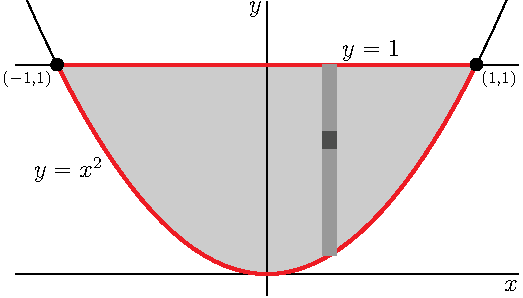
\includegraphics{fig/OE05D_7.pdf}
\end{center}

By definition, the centre of mass is $(\bar x, \bar y)$,
with $\bar x$ and $\bar y$ being the weighted averages  of the $x$ and 
$y$--coordinates, respectively, over $D$. That is,
\begin{align*}
\bar x = \frac{\dblInt_D x\ \rho(x,y)\ \dee{A}}{\dblInt_D \rho(x,y)\ \dee{A}}
\qquad
\bar y = \frac{\dblInt_D y\ \rho(x,y)\ \dee{A}}{\dblInt_D \rho(x,y)\ \dee{A}}
\end{align*}
By symmetry under reflection in the $y$--axis, we have $\bar x=0$.
So we just have to determine $\bar y$. 
We'll evaluate the integrals using vertical strips as in the figure above.
Looking at that figure, we see that
\begin{itemize}
\item 
$x$ runs from $-1$ to $1$, and
\item
for each fixed $x$ in that range, $y$ runs from $x^2$ to $1$.
\end{itemize}
So the denominator is
\begin{align*}
\dblInt_D \rho(x,y)\ \dee{A}
&= \int_{-1}^1\dee{x}\int_{x^2}^1\dee{y}\ \overbrace{y}^{\rho(x,y)} \\
&= \frac{1}{2}\int_{-1}^1 \dee{x}\ (1-x^4)
 =\int_0^1 \dee{x}\ (1-x^4) \\
&=\frac{4}{5}
\end{align*}
and the numerator of $\bar y$ is
\begin{align*}
\dblInt_D y\,\rho(x,y)\ \dee{A}
&= \int_{-1}^1\dee{x}\int_{x^2}^1\dee{y}\ y\overbrace{y}^{\rho(x,y)} \\
&= \frac{1}{3}\int_{-1}^1 \dee{x}\ (1-x^6)
 =\frac{2}{3}\int_0^1 \dee{x}\ (1-x^6) \\
&=\frac{2}{3}\ \frac{6}{7} = \frac{4}{7}
\end{align*}
All together, $\bar x=0$ and
\begin{align*}
\bar y = \frac{\frac{4}{7}} {\frac{4}{5}}
       =  \frac{5}{7}
\end{align*}
\end{solution}

%%%%%%%%%%%%%%%%%%%%%%%%%%%%%%%%
\begin{question}[M200 2008D] %7
Let R be the region bounded on the left by $x = 1$ and on the right
by $x^2 + y^2 = 4$. The density in $R$ is
\begin{equation*}
\rho(x,y) =\frac{1}{\sqrt{x^2+y^2}}
\end{equation*} 
\begin{enumerate}[(a)]
\item
Sketch the region $R$.

\item
Find the mass of $R$.

\item
Find the centre-of-mass of $R$.

\end{enumerate}

Note: You may use the result $\int \sec(\theta)\ \dee{\theta} 
= \ln |\sec \theta + \tan \theta| + C$.
\end{question}

%\begin{hint}
%
%\end{hint}

\begin{answer}
(a)
\begin{center}
     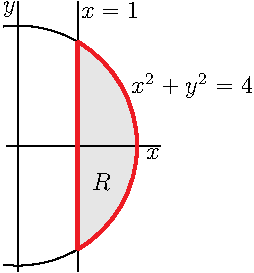
\includegraphics{fig/OE08D_7.pdf}
\end{center}
(b) $\text{mass} = \frac{4\pi}{3} - 2\ln\big(2+\sqrt{3}\big)$

(c)
$\bar x = \frac{2\sqrt{3}- \ln(2+\sqrt{3})}
            {\frac{4\pi}{3} - 2\ln(2+\sqrt{3})}
        \approx 1.38$,
$\bar y=0$.
\end{answer}

\begin{solution}
(a) Here is a sketch of $R$.
\begin{center}
     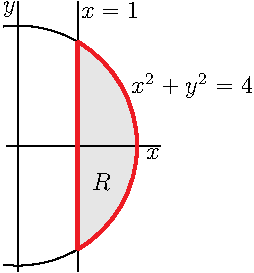
\includegraphics{fig/OE08D_7.pdf}
\end{center}

(b) Considering that
\begin{itemize}
\item
$\rho(x,y)$ is invariant under rotations about the origin and
\item
the outer curve $x^2+y^2=4$  is invariant under rotations about the origin and
\item
the given hint involves a $\theta$ integral
\end{itemize}
we'll use polar coordinates. 

Observe that the line $x=1$ and the circle $x^2+y^2=4$ 
intersect when
\begin{equation*}
1+y^2=4 
\iff y=\pm\sqrt{3}
\end{equation*}
and that the polar coordinates of the point $(x,y)=\big(1,\sqrt{3}\big)$
are $r=\sqrt{x^2+y^2}=2$ and $\theta=\arctan\frac{y}{x}=\arctan \sqrt{3}
=\frac{\pi}{3}$. Looking at the sketch 
\begin{center}
     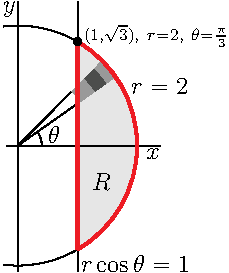
\includegraphics{fig/OE08D_7w.pdf}
\end{center}
we see that, on $R$,
\begin{itemize}
\item
$\theta$ runs from $-\frac{\pi}{3}$ to $\frac{\pi}{3}$ and
\item
for each fixed $\theta$ in that range, $r$ runs from $\frac{1}{\cos\theta}
=\sec\theta$ to $2$.
\item
In polar coordinates, $\dee{A}=r\,\dee{r}\,\dee{\theta}$, and
\item 
the density $\rho =\frac{1}{\sqrt{x^2+y^2}} =\frac{1}{r}$
\end{itemize}
So the mass is
\begin{align*}
M&=\dblInt_R \rho(x,y)\ \dee{A}
=\int_{-\pi/3}^{\pi/3}\dee{\theta}\int_{\sec\theta}^2\dee{r}\ \frac{r}{r}
=\int_{-\pi/3}^{\pi/3}\dee{\theta}\ \big[2-\sec\theta\big] \\
&=2\int_0^{\pi/3}\dee{\theta}\ \big[2-\sec\theta\big] \\
&= 2\Big[2\theta - \ln\big(\sec\theta+\tan\theta\big)\Big]_0^{\pi/3} \\
&= 2\left[\frac{2\pi}{3} - \ln\big(2+\sqrt{3}\big)
            + \ln\big(1+0\big)\right] \\
&= \frac{4\pi}{3} - 2\ln\big(2+\sqrt{3}\big)
\end{align*}


(c)
By definition, the centre of mass is $(\bar x, \bar y)$,
with $\bar x$ and $\bar y$ being the weighted averages  of the $x$ and 
$y$--coordinates, respectively, over $R$. That is,
\begin{align*}
\bar x = \frac{\dblInt_R x\ \rho(x,y)\ \dee{A}}{\dblInt_R \rho(x,y)\ \dee{A}}
\qquad
\bar y = \frac{\dblInt_R y\ \rho(x,y)\ \dee{A}}{\dblInt_R \rho(x,y)\ \dee{A}}
\end{align*}
By symmetry under reflection in the $x$--axis, we have $\bar y=0$.
So we just have to determine $\bar x$. 
The numerator is
\begin{align*}
\dblInt_R x\ \rho(x,y)\ \dee{A}
&=\int_{-\pi/3}^{\pi/3}\dee{\theta}\int_{\sec\theta}^2\dee{r}\ \frac{r}{r}\ 
       \overbrace{r\cos\theta}^{x} \\
&=\frac{1}{2}\int_{-\pi/3}^{\pi/3}\dee{\theta}\ \big[4-\sec^2\theta\big]
                               \cos\theta 
=\int_0^{\pi/3}\dee{\theta}\ \big[4\cos\theta-\sec\theta\big] \\
&= \Big[4\sin\theta - \ln\big(\sec\theta+\tan\theta\big)\Big]_0^{\pi/3} \\
&= \left[4\frac{\sqrt{3}}{2} - \ln\big(2+\sqrt{3}\big)
            + \ln\big(1+0\big)\right] \\
&=  2\sqrt{3}- \ln\big(2+\sqrt{3}\big)
\end{align*}
All together, $\bar y=0$ and
\begin{align*}
\bar x = \frac{2\sqrt{3}- \ln\big(2+\sqrt{3}\big)}
            {\frac{4\pi}{3} - 2\ln\big(2+\sqrt{3}\big)}
        \approx 1.38
\end{align*}
\end{solution}

%%%%%%%%%%%%%%%%%%%%%%%%%%%%%%%%
\begin{question}[M200 2009D] %7
A thin plate of uniform density $1$ is bounded by the positive $x$ and $y$ 
axes and the cardioid $\sqrt{x^2+y^2}=r=1+\sin\theta$, which is given
in polar coordinates. Find the $x$--coordinate of its centre of mass.
\end{question}

%\begin{hint}
%
%\end{hint}

\begin{answer}
$\bar x = \frac{10}{3\pi+8} \approx 0.57$
\end{answer}

\begin{solution}
Let's call the plate $\cP$. By definition, the $x$--coordinate of its 
centre of mass is
\begin{align*}
\bar x = \frac{\dblInt_\cP x\ \dee{A}}{\dblInt_\cP\dee{A}}
\end{align*}
Here is a sketch of the plate.
\begin{center}
     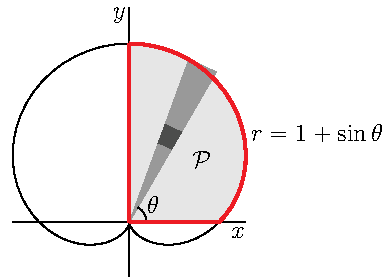
\includegraphics{fig/OE09D_7.pdf}
\end{center}
The cardiod is given to us in polar coordinates, so let's evaluate the
integrals in polar coordinates. Looking at the sketch above, we see that,
on $\cP$,
\begin{itemize}
\item
$\theta$ runs from $0$ to $\pi/2$ and
\item
for each fixed $\theta$ in that range, $r$ runs from $0$
to $1+\sin\theta$.
\item
In polar coordinates $\dee{A} = r\,\dee{r}\,\dee{\theta}$
\end{itemize}
So the two integrals of interest are
\begin{align*}
\dblInt_\cP\dee{A}
&=\int_0^{\pi/2}\dee{\theta}\int_0^{1+\sin\theta}\dee{r}\ r \\
&=\frac{1}{2} \int_0^{\pi/2}\dee{\theta}\ \big(1+2\sin\theta +\sin^2\theta\big)\\
&=\frac{1}{2}\frac{\pi}{2} +\Big[-\cos\theta\Big]_0^{\pi/2}
+\frac{1}{2} \int_0^{\pi/2}\dee{\theta}\ \frac{1-\cos(2\theta)}{2} \\
&=\frac{\pi}{4} + 1 
    +\frac{1}{4}\left[\theta-\frac{\sin(2\theta)}{2}\right]_0^{\pi/2} \\
&=\frac{3\pi}{8} + 1
\end{align*}
and
\begin{align*}
\dblInt_\cP x\ \dee{A}
&=\int_0^{\pi/2}\dee{\theta}\int_0^{1+\sin\theta}\dee{r}\ r
   \overbrace{(r\cos\theta)}^{x} \\
&=\frac{1}{3} \int_0^{\pi/2}\dee{\theta}\ \big(1+\sin\theta\big)^3\cos\theta\\
&=\frac{1}{3}\int_1^2\dee{u}\ u^3\qquad\text{with }u=1+\sin\theta,\ 
                                       \dee{u} = \cos\theta\,\dee{\theta}  \\
&=\frac{1}{12}\big[2^4-1^4\big] \\
&=\frac{5}{4}
\end{align*}
All together
\begin{align*}
\bar x = \frac{\frac{5}{4}}{\frac{3\pi}{8} + 1}
=\frac{10}{3\pi+8}
\approx 0.57
%0.573895405
\end{align*}
For an efficient, sneaky, way to evaluate  
$\int_0^{\pi/2}\sin^2\theta\ \dee{\theta}$,
see Remark \eref{CLP200}{rem sneaky} in the CLP-3 text.
\end{solution}

%%%%%%%%%%%%%%%%%%%%%%%%%%%%%%%%
\begin{question}[M200 2010A] %7
A thin plate of uniform density $k$ is bounded by the positive $x$ and $y$ 
axes and the circle $x^2 + y^2 = 1$. Find its centre of mass.
\end{question}

%\begin{hint}
%
%\end{hint}

\begin{answer}
$\bar x = \bar y =\frac{4}{3\pi}$
\end{answer}

\begin{solution}
 Call the plate $P$. 
By definition, the centre of mass is $(\bar x, \bar y)$,
with $\bar x$ and $\bar y$ being the weighted averages  of the $x$ and 
$y$--coordinates, respectively, over $P$. That is,
\begin{align*}
\bar x = \frac{\dblInt_P x\ \rho(x,y)\ \dee{A}}{\dblInt_P \rho(x,y)\ \dee{A}}
\qquad
\bar y = \frac{\dblInt_P y\ \rho(x,y)\ \dee{A}}{\dblInt_P \rho(x,y)\ \dee{A}}
\end{align*}
with $\rho(x,y)=k$.
Here is a sketch of $P$.
\begin{center}
     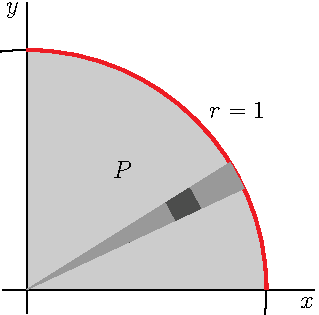
\includegraphics{fig/OE10A_7.pdf}
\end{center}
By symmetry under reflection in the line $y=x$, we have $\bar y=\bar x$.
So we just have to determine 
\begin{equation*}
\bar x = \frac{\dblInt_P x\ \dee{A}}{\dblInt_P  \dee{A}}
\end{equation*}
The denominator is just one quarter of the area of circular disk of radius $1$.
That is, $\dblInt_P  \dee{A}=\frac{\pi}{4}$.
We'll evaluate the numerator using polar coordinates as in the figure above.
Looking at that figure, we see that
\begin{itemize}
\item 
$\theta$ runs from $0$ to $\frac{\pi}{2}$, and
\item
for each fixed $\theta$ in that range, $r$ runs from $0$ to $1$.
\end{itemize}
As $\dee{A}=r\,\dee{r}\,\dee{\theta}$, and $x=r\cos\theta$, the numerator
\begin{align*}
\dblInt_P x\ \dee{A}
&=\int_0^{\pi/2}\dee{\theta} \int_0^1\dee{r}\ r\overbrace{r\cos\theta}^{x}
=\left[\int_0^{\pi/2}\dee{\theta}\ \cos\theta\right]
 \left[ \int_0^1\dee{r}\ r^2\right] \\
&=\Big[\sin\theta\Big]_0^{\pi/2} \left[\frac{r^3}{3}\right]_0^1 \\
&=\frac{1}{3}
\end{align*}

All together
\begin{align*}
\bar x = \bar y = \frac{1/3}{\pi/4} =\frac{4}{3\pi}
\end{align*}
\end{solution}

%%%%%%%%%%%%%%%%%%%%%%%%%%%%%%%%
\begin{question}[M200 2011D] %6
Let $R$ be the triangle with vertices $(0, 2)$, $(1, 0)$, and $(2, 0)$. 
Let $R$ have density  $\rho(x, y) = y^2$.
Find $\bar y$, the $y$--coordinate of the center of mass of $R$. 
You do not need to find $\bar x$.
\end{question}

%\begin{hint}
%
%\end{hint}

\begin{answer}
$\frac{6}{5}$
\end{answer}

\begin{solution}
Here is a sketch of $R$.
\begin{center}
     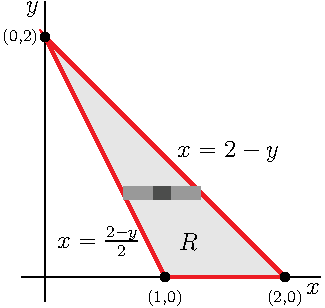
\includegraphics{fig/OE11D_6.pdf}
\end{center}
Note that
\begin{itemize}
\item
 the equation of the straight line through $(2,0)$ and $(0,2)$
 is $y=2-x$, or $x=2-y$. (As a check note that both points $(2,0)$ and $(0,2)$
  are on $x=2-y$.
\item
 The equation of the straight line through $(1,0)$ and $(0,2)$
 is $y=2-2x$, or $x=\frac{2-y}{2}$. (As a check note that both points 
 $(0,2)$ and $(1,0)$ are on $x=\frac{2-y}{2}$.
\end{itemize}
By definition, the $y$--coordinate of the center of mass of $R$
is the weighted average of $y$ over $R$, which is
\begin{equation*}
\bar y =\frac{\dblInt_R y\,\rho(x,y)\,\dee{A}}{\dblInt_R \rho(x,y)\,\dee{A}}
       =\frac{\dblInt_R y^3\,\dee{A}}{\dblInt_R y^2\,\dee{A}}
\end{equation*} 
On $R$,
\begin{itemize}
\item
$y$ runs from $0$ to $2$. That is, $0\le y\le 2$.
\item
For each fixed $y$ in that range, $x$ runs from $\frac{2-y}{2}$ to
$2-y$. In inequalities, that is $\frac{2-y}{2}\le x\le 2-y$.
\end{itemize}
Thus
\begin{equation*}
R = \left\{\ (x,y)\ \left|\ 0\le y\le 2,\ \frac{2-y}{2}\le x\le 2-y
                                     \right.\right\}
\end{equation*}

For both $n=2$ and $n=3$, we have
\begin{align*}
\dblInt_R y^n\,\dee{A}
&=\int_0^2\dee{y} \int_{\frac{2-y}{2}}^{2-y}\dee{x}\ y^n \\
&=\int_0^2\dee{y} \ y^n\frac{2-y}{2} \\
&=\frac{1}{2}\left[\frac{2y^{n+1}}{n+1}-\frac{y^{n+2}}{n+2}\right]_0^2 \\
&=\frac{1}{2}\left[\frac{2^{n+2}}{n+1}-\frac{2^{n+2}}{n+2}\right] \\
&=\frac{2^{n+1}}{(n+1)(n+2)}
\end{align*}
So 
\begin{align*}
\bar y =\frac{\dblInt_R y^3\,\dee{A}}{\dblInt_R y^2\,\dee{A}}
       =\frac{ \frac{2^4}{(4)(5)} }{ \frac{2^{3}}{(3)(4)} }
       =\frac{6}{5}
\end{align*}
\end{solution}

%%%%%%%%%%%%%%%%%%%%%%%%%%%%%%%%
\begin{question}[M200 2012A] %7
The average distance of a point in a plane region $D$ to a point $(a, b)$ is defined by
\begin{equation*}
\frac{1}{A(D)}\dblInt_D \sqrt{(x-a)^2+(y-b)^2}\ \dee{x}\,\dee{y}
\end{equation*}
where $A(D)$ is the area of the plane region $D$. Let $D$ be the unit disk 
$1 \ge x^2 + y^2$.
Find the average distance of a point in $D$ to the center of $D$.
\end{question}

%\begin{hint}
%
%\end{hint}

\begin{answer}
$\frac{2}{3}$
\end{answer}

\begin{solution}
By the definition given in the statement with $(a,b)=(0,0)$,
the average is
\begin{align*}
\frac{1}{A(D)}\dblInt_D \sqrt{x^2+y^2}\ \dee{x}\,\dee{y}
\end{align*}
The denominator $A(D) = \pi$. We'll use polar coordinates to evaluate the
numerator.
\begin{align*}
\dblInt_D \sqrt{x^2+y^2}\ \dee{x}\,\dee{y}
&=\int_0^{2\pi}\dee{\theta}\int_0^1\dee{r}
     \ r\sqrt{r^2\cos^2\theta+r^2\sin^2\theta} \\
&=\int_0^{2\pi}\dee{\theta}\int_0^1\dee{r}\ r^2 
=\int_0^{2\pi}\dee{\theta}\ \frac{1}{3} \\
&=\frac{2\pi}{3}
\end{align*}
So the average is
\begin{equation*}
\frac{\frac{2\pi}{3}}{\pi}=\frac{2}{3}
\end{equation*}
\end{solution}

%%%%%%%%%%%%%%%%%%%%%%%%%%%%%%%%
\begin{question}[M200 2012D] %8
A metal crescent is obtained by removing the interior of the circle defined by 
the equation $x^2 + y^2 = x$ from the metal plate of constant density 1 
occupying the unit disc $x^2 + y^2 \le 1$.
\begin{enumerate}[(a)]
\item
Find the total mass of the crescent.
\item
Find the $x$-coordinate of its center of mass.
\end{enumerate}

You may use the fact that 
$\int_{-\pi/2}^{\pi/2}\cos^4(\theta)\ \dee{\theta}=\frac{3\pi}{8}$.
\end{question}

%\begin{hint}
%
%\end{hint}

\begin{answer}
(a) $\frac{3\pi}{4}$\qquad
(b) $-\frac{1}{6}$
\end{answer}

\begin{solution}
Note that $x^2+y^2=x$ is equivalent to
$\left(x-\frac{1}{2}\right)^2+y^2=\frac{1}{4}$, which is the
circle of radius $\frac{1}{2}$ centred on $\left(\frac{1}{2},0\right)$.
Let's call the crescent $\cC$ and write
\begin{align*}
D &= \Set{(x,y)}{x^2+y^2\le 1} \\
H &= \Set{(x,y)}{\left(x-\tfrac{1}{2}\right)^2+y^2\le\tfrac{1}{4}}
\end{align*}
so that
\begin{equation*}
\cC= D\setminus H
\end{equation*}
meaning that $\cC$ is the disk $D$ with the ``hole'' $H$ removed.
Here is a sketch.

\begin{center}
     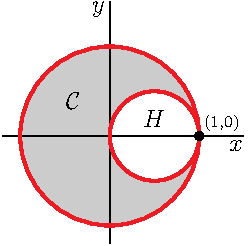
\includegraphics{fig/OE12D_8.pdf}
\end{center}

(a) As $D$ is a disk of radius $1$, it has area $\pi$.
    As $H$ is a disk of radius $\nicefrac{1}{2}$, it has 
           area $\nicefrac{\pi}{4}$.
As $\cC$ has density $1$, 
\begin{align*}
\text{Mass}(\cC) &= \dblInt_\cC \dee{A}
                  = \dblInt_D\dee{A} -\dblInt_H\dee{A} \\
   &=\pi - \frac{\pi}{4} \\
   &=\frac{3\pi}{4}
\end{align*}



(b)
Recall that, by definition, the $x$--coordinate of the centre of mass
of $\cC$ is the average value of $x$ over $\cC$, which is
\begin{align*}
\bar x = \frac{\dblInt_\cC x\,\dee{A}}{\dblInt_\cC \dee{A}}
\end{align*}
We have already found that $\dblInt_\cC \dee{A}=\frac{3\pi}{4}$. 
So we have to determine the numerator
\begin{equation*}
\dblInt_\cC x\,\dee{A} = \dblInt_D x\,\dee{A} - \dblInt_H x\,\dee{A}
\end{equation*}
As $x$ is an odd function and $D$ is invariant under $x\rightarrow -x$,
$\dblInt_D x\,\dee{A}=0$. So we just have to determine 
$\dblInt_H x\,\dee{A}$.
To do so we'll work in polar coordinates, so that 
$\dee{A} = r\,\dee{r}\,\dee{\theta}$.
In polar coordinates $x^2 + y^2 = x$ is $r^2 =r\cos\theta$
or $r=\cos\theta$. So, looking at the figure above (just before the 
solution to part (a)), on the domain of integration,
\begin{itemize}
\item
$\theta$ runs from $-\frac{\pi}{2}$ to $\frac{\pi}{2}$. 
\item
For each fixed $\theta$ in that range, $r$ runs from $0$ to
$\cos\theta$.
\end{itemize}
So the integral is
\begin{align*}
\dblInt_H x\,\dee{A}
   &= \int_{-\pi/2}^{\pi/2}\dee{\theta}\int_0^{\cos\theta}\dee{r}\ 
           r\overbrace{(r\cos\theta)}^{x} \\
   &=\int_{-\pi/2}^{\pi/2}\dee{\theta} \ \frac{\cos^4\theta}{3} \\
   &= \frac{\pi}{8}
\end{align*}
So all together
\begin{align*}
\bar x = \frac{\dblInt_\cC x\,\dee{A}}{\dblInt_\cC \dee{A}}
       = \frac{\dblInt_D x\,\dee{A} - \dblInt_H x\,\dee{A}}{\dblInt_\cC \dee{A}}
       =\frac{0-\frac{\pi}{8}}{\frac{3\pi}{4}}
       =-\frac{1}{6}
\end{align*}
\end{solution}

%%%%%%%%%%%%%%%%%%%%%%%%%%%%%%%%
\begin{question}[M200 2002D] %7
Let $D$ be the region in the $xy$--plane which is inside
the circle $x^2+(y-1)^2=1$ but outside the circle $x^2+y^2=2$. Determine
the mass of this region if the density is given by 
$$
\rho(x,y)=\frac{2}{\sqrt{x^2+y^2}}
$$
\end{question}

\begin{hint}
Try using polar coordinates.
\end{hint}

\begin{answer}
$4\sqrt{2} -\sqrt{2}\pi\approx 1.214$
\end{answer}

\begin{solution}
The domain is pictured below.
\begin{center}
     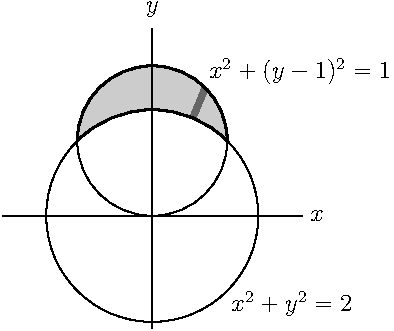
\includegraphics{fig/OE02DQ7.pdf}
\end{center}
The two circles intersect when $x^2+y^2=2$ and
\begin{align*}
x^2+(y-1)^2=2-y^2+(y-1)^2=1
%\iff y^2-(y-1)^2=1
\iff -2y+3=1\iff y=1\text{ and } x=\pm 1
\end{align*}
In polar coordinates $x^2+y^2=2$ is $r=\sqrt{2}$ and 
$x^2+(y-1)^2=x^2+y^2-2y+1=1$ is $r^2-2r\sin\theta=0$ or $r=2\sin\theta$.
The two curves intersect when $r=\sqrt{2}$ and$\sqrt{2}=2\sin\theta$ so that 
$\theta=\frac{\pi}{4}$ or $\frac{3}{4}\pi$. So 
\begin{equation*}
D=\Set{(r\cos\theta,r\sin\theta)}{\tfrac{1}{4}\pi\le\theta\le\tfrac{3}{4}\pi,\ 
          \sqrt{2}\le r\le 2\sin\theta}
\end{equation*}
and, as the density is $\frac{2}{r}$,
\begin{align*}
\text{mass}
&=\int_{\pi/4}^{3\pi/4}\dee{\theta}\int^{2\sin\theta}_{\sqrt{2}}\dee{r}\ 
          r\frac{2}{r}
=2\int_{\pi/4}^{3\pi/4}\dee{\theta}\ \big[2\sin\theta -\sqrt{2}\,\big]
=4\int_{\pi/4}^{\pi/2}\dee{\theta}\ \big[2\sin\theta -\sqrt{2}\,\big] \cr
&=4\Big[-2\cos\theta -\sqrt{2}\theta\Big] _{\pi/4}^{\pi/2}
=4\sqrt{2} -\sqrt{2}\pi\approx 1.214
\end{align*}
\end{solution}


%%%%%%%%%%%%%%%%%%
\subsection*{\Application}
%%%%%%%%%%%%%%%%%%

%%%%%%%%%%%%%%%%%%%%%%%%%%%%%%%%
\begin{question}[M200 2003A] %6
Let $a$, $b$ and $c$ be positive numbers, and let $T$ be
the triangle whose vertices are $(-a,0)$, $(b,0)$ and $(0,c)$.
\begin{enumerate}[(a)]
\item 
Assuming that the density is constant on $T$, find the center
of mass of $T$.

\item 
The medians of $T$ are the line segments which join a vertex
of $T$ to the midpoint of the opposite side. It is a well known fact that the
three medians of any triangle meet at a point, which is known as the centroid
of $T$. Show that the centroid of $T$ is its centre of mass.
\end{enumerate}
\end{question}

%\begin{hint}
%
%\end{hint}

\begin{answer}
(a) $\frac{1}{3}(b-a\,,\,c)$\qquad
(b) See the solution.
\end{answer}

\begin{solution}
(a) The side of the triangle from $(-a,0)$ to $(0,c)$ is straight line that passes through those two points. As $y=0$ when $x=-a$, the line must have 
an equation of the form $y=K(x+a)$ for some constant $K$. Since $y=c$ when
$x=0$, the constant $K=\frac{c}{a}$. So that the equation is 
$y=\frac{c}{a}(x+a)$.
has equation $cx-ay=-ac$. Similarly the side of the triangle from 
$(b,0)$ to $(0,c)$ has equation $y=\frac{c}{b}(b-x)$. 
The triangle has area $A=\frac{1}{2}(a+b)c$. It has centre
of mass $(\bar x,\bar y)$ with
\begin{align*}
\bar x=\frac{1}{A}\dblInt_T x\ \dee{x}\dee{y}\qquad
\bar y=\frac{1}{A}\dblInt_T y\ \dee{x}\dee{y}
\end{align*}
To evaluate the integrals we'll decompose the triangle into vertical strips
as in the figure
\begin{center}
     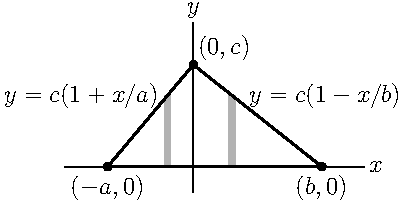
\includegraphics{fig/OE03AQ6a.pdf}
\end{center}
\begin{align*}
\bar x&=\frac{1}{A}\dblInt_T x\ \dee{x}\dee{y} \\
&=\frac{1}{A}\bigg(\int_{-a}^0 \dee{x}\int_0^{c+{c\over a}x}\dee{y}\ x
                   +\int_0^b \dee{x}\int_0^{c-{c\over b}x}\dee{y}\ x\bigg)\\
&=\frac{1}{A}\bigg(\int_{-a}^0 \dee{x}\ x\left(c+\frac{c}{a}x\right)
                   +\int_0^b \dee{x}\ x\left(c-\frac{c}{b}x\right)\bigg)\\
&=\frac{1}{A}\left(\left[\frac{1}{2} cx^2+\frac{c}{3a}x^3\right]_{-a}^0 
                   +\left[\frac{1}{2} cx^2-\frac{c}{3b}x^3\right]_0^b\right) \\
&=2\frac{\frac{1}{2} c(b^2-a^2)+\frac{c}{3}(a^2-b^2)}{(a+b)c}
=\frac{1}{3}(b-a)\\
\bar y&=\frac{1}{A}\dblInt_T y\ \dee{x}\dee{y} \\
&=\frac{1}{A}\bigg(\int_{-a}^0 \dee{x}\int_0^{c+{c\over a}x}\dee{y}\ y
                   +\int_0^b \dee{x}\int_0^{c-{c\over b}x}\dee{y}\ y\bigg)\\
&=\frac{1}{A}\bigg(\int_{-a}^0 \dee{x}\ \frac{1}{2}\left(c+\frac{c}{a}x\right)^2
                   +\int_0^b \dee{x}\ \frac{1}{2}\left(c-\frac{c}{b}x\right)^2\bigg)\\
&=\frac{1}{A}\left(\frac{a}{6c}\left[c+\frac{c}{a}x\right]^3\bigg|_{-a}^0 
                   -\frac{b}{6c}\left(c-\frac{c}{b}x\right)^3\bigg|_0^b\,
               \right) \\
&=2\frac{\frac{ac^2}{6}+\frac{bc^2}{6}}{(a+b)c}
=\frac{c}{3}
\end{align*}

(b) The midpoint of the side opposite $(-a,0)$ is $\frac{1}{2}\big[(b,0)+(0,c)\big]=\frac{1}{2}(b,c)$.
The vector from $(-a,0)$ to $\frac{1}{2}(b,c)$ is $ \frac{1}{2}\llt b,c\rgt-\llt-a,0\rgt
=\llt a+\frac{b}{2},\frac{c}{2}\rgt$. So
the line joining these two points has vector parametric equation
\begin{equation*}
\vr(t)=\llt -a,0\rgt+t\llt a+\frac{1}{2} b\,,\,\frac{1}{2} c\rgt
\end{equation*}
\begin{center}
     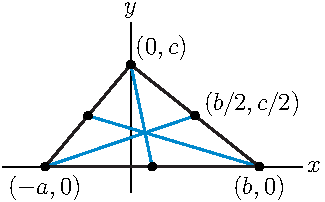
\includegraphics{fig/OE03AQ6.pdf}
\end{center}
The point $(\bar x,\bar y)$ lies on this line since
\begin{equation*}
\vr\left(\frac{2}{3}\right)=\left(\frac{1}{3}(b-a)\,,\,\frac{c}{3}\right)
=(\bar x,\bar y)
\end{equation*}
Similarly, the midpoint of the side opposite $(b,0)$ is $\frac{1}{2}(-a,c)$.
The line joining these two points has vector parametric equation
\begin{equation*}
\vr(t)=\llt b,0\rgt +t\llt-b-\frac{1}{2} a\,,\,\frac{1}{2} c\rgt
\end{equation*}
The point $(\bar x,\bar y)$ lies on this line too, since
\begin{equation*}
\vr\left(\frac{2}{3}\right)=\left(\frac{1}{3}(b-a),\frac{c}{3}\right)
=(\bar x,\bar y)
\end{equation*}
It is not really necessary to check that $(\bar x,\bar y)$ lies on the
third median, but let's do it anyway. The midpoint of the side opposite $(0,c)$ is $\frac{1}{2}(b-a,0)$.
The line joining these two points has vector parametric equation
\begin{equation*}
\vr(t)=\llt 0,c\rgt+t\llt\frac{b}{2}-\frac{a}{2},-c\rgt
\end{equation*}
The point $(\bar x,\bar y)$ lies on this median too, since
\begin{equation*}
\vr\left(\frac{2}{3}\right)=\left(\frac{1}{3}(b-a),\frac{c}{3}\right)
=(\bar x,\bar y)
\end{equation*}
\end{solution}